\documentclass[]{extarticle}

\usepackage[]{fancyhdr}
\usepackage[french]{babel}
\usepackage[svgnames, table]{xcolor}
\usepackage[]{geometry}
\usepackage[]{graphicx}

\pagestyle{fancy}
\fancyhead[L]{The Believer's Quest}
\geometry{hmargin=3cm,vmargin=2.5cm}

\begin{document}
\textsc{ }\\
\textsc{ }\\
\textsc{ }\\
\textsc{ }\\
\textsc{ }\\

\begin{center}
\textsc{\LARGE Cahier des Charges} \\
\bigbreak
\bigbreak
\bigbreak
\textsc{\Huge The Believer's Quest}
\bigbreak
\bigbreak
\bigbreak
\bigbreak
\bigbreak
\bigbreak
\bigbreak
\bigbreak
\bigbreak
\bigbreak
\bigbreak
\bigbreak
\bigbreak
par \\
\[MSN^{2}\]\\
Maxence PLANTARD, Sarah GUTIEREZ \\
Nicolas INDJEIN, Nicolas LORRAIN \\
\bigbreak
\bigbreak
\bigbreak
PROJET S2 2019
\end{center}
\newpage

\renewcommand{\contentsname}{Sommaire}
\tableofcontents
\newpage

\section{Introduction}

\bigbreak
\bigbreak
Ce projet est un jeu de type rogue-like hybride 2D. Le rogue-like est un genre de jeux vidéo dont le gameplay est inspiré de Rogue, sorti sur Berkeley Unix en 1980. Le principe est généralement d’explorer un donjon dont les salles sont générées de manière procédurale. La progression est basée sur la mort du joueur. Chaque fois que celui-ci meurt il perd presque tous les objets obtenus pendant la partie. Certains objets sont conservés pour améliorer les compétences du personnage et son armement notamment dans un magasin mis à la disposition du joueur avant une nouvelle partie.
\bigbreak
Nous nous sommes inspirés de jeux comme The Binding of Isaac, Dead Cells ou encore Enter The Gungeon. Certains membres du groupe ayant déjà joué à ce type de jeu, et le concept étant original nous avons décidé de nous orienter vers cette idée. L’organisation avec des salles carrées provient notamment de Isaac, quant au système d’armes et d’objets il nous est inspiré de jeux comme Enter The Gungeon.
\bigbreak
Nous aspirons, à la fin de notre projet, à être plus informé vis-à-vis du processus de création de certains de ces jeux. Ce projet formateur permet d’appréhender le travail en équipe qu’effectue un ingénieur au quotidien. De plus, en cherchant à développer notre projet nous gagnons en expérience sur certains logiciels comme Unity ou FL Studio pour la partie sonore. Chacun développe ses compétences mais observe aussi le travail des autres et se renseigne sur les logiciels utilisés. La confrontation à un projet de cette taille avec des limites de temps pour le rendu nous apprend à travailler efficacement en divisant les tâches.
\bigbreak
Le but premier reste cependant de proposer aux utilisateurs un jeu à la fois ludique et complet. L’instauration d’un contenu riche et varié est notre priorité pour répondre à cette problématique. Les ressources audiovisuelles seront majoritairement issues de notre créativité et notre travail afin de rendre le jeu unique et de découvrir d’autres aspects de la création artistique d’un jeu.

\newpage
\section{Les membres du groupe}
	\subsection{Présentation du groupe}
\bigbreak
\bigbreak
Notre groupe est composé de quatre membres. Nous nous sommes regroupés car nous nous entendons très bien et nous avions vraiment envie de travailler tous ensemble sur The Believer’s Quest. Deux d’entre nous se connaissaient avant EPITA mais notre groupe s’est vraiment formé et soudé à partir de cette première année. Notre groupe est basé sur de la complicité, de la confiance et assez de sérieux pour mener à bien notre projet.
\bigbreak
	\subsection{Apports personnels}
		\subsubsection{Sarah GUTIEREZ}
\bigbreak
\bigbreak
Ma passion pour l’informatique s’est développée quand j’étais assez jeune. J’ai toujours été fascinée par le fonctionnement des ordinateurs et de tout ce qui est lié à ceux-ci. Je suis aussi une très grande fan de jeux vidéo, films, séries, comics et musique. J’ai vraiment commencé à programmer il y a à peu près un an et demi, en attaquant le Java et le HTML. Depuis mon année de troisième je savais que je voulais travailler dans l’informatique et maintenant je suis à EPITA! Ce n’est pas le premier gros projet que je réalise mais celui-ci est spécial car c’est un jeu-vidéo.  

La réalisation de ce projet me sera très bénéfique car c’est avant tout un travail d’équipe. Celui-ci permet d’être plus efficace et plus instructif car en aidant les autres, on apprend aussi avec eux. Personnellement, travailler sur ce projet me permettra aussi de comprendre quelles sont les responsabilités mises en jeu.

Ce projet va aussi nous aider à mieux comprendre comment créer de A à Z un jeu vidéo. Je trouve ça extrêmement intéressant, notamment tout le processus de réflexion sur notre sujet pour savoir quels moyens nous allons mettre en œuvre pour arriver à un jeu qui correspond exactement à notre idée de base.
De mon côté, ce projet va m’apporter de nouvelles connaissances en programmation. Je vais pouvoir approfondir mes compétences en développement Web mais aussi en C\# et, bien sûr, apprendre à utiliser le logiciel Unity. Quand on programme un nouveau jeu on part d’une base vide et on construit tout. Tout ne fonctionnera pas du premier coup et il y aura sûrement de nombreux problèmes dans notre code mais c’est ce qui rend tout notre travail palpitant.
\bigbreak
		\subsubsection{Maxence PLANTARD}
\bigbreak
\bigbreak
	Ma passion pour l’informatique n’est pas récente. En effet, étant joueur depuis mon plus jeune âge je me suis très vite intéressé à différents langages de programmation comme le python ou le C. Néanmoins j’ai réellement commencé à travailler sur python en première. J’ai continué à étudier Caml et Python en prépa avant de me tourner vers Epita pour étudier plus en profondeur l’algorithmique et les langages informatiques. Le code ne reste cependant pas mon occupation première. Je préfère utiliser des logiciels divers liés au monde du numérique comme FL Studio pour la musique. J’espère pouvoir mieux comprendre les logiciels et les jeux auxquels je joue après ce projet qui sera mon premier vrai projet.
	
Les mathématiques étant une de mes grandes passions j’espère pouvoir apporter à mon groupe une aide importante lors de la résolution de problème logique comme pour le calcul de probabilité ou autre prévision d’événement. Je me charge de créer la musique du jeu et les bruitages ce qui coïncide avec l’intérêt  que j’apporte à ce domaine. La création ex nihilo de notre jeu va nous pousser à acquérir de nouvelles compétences notamment pour résoudre les problèmes en respectant les délais impartis.

\bigbreak
	 	\subsubsection{Nicolas INDJEIN}
\bigbreak
\bigbreak
	J'ai vraiment commencé à m'intéresser à la programmation informatique il y a 2 ans. J'aime bien comprendre comment les choses fonctionnent et depuis bien longtemps je souhaite réaliser un jeu vidéo par moi-même. Ce projet va me permettre d’évoluer sur plusieurs points. Tout d’abord, la partie graphique va me permettre d’améliorer mes compétences en dessin et me faire découvrir une nouvelle manière de dessiner. En effet je n’ai jamais vraiment touché au pixel art.
	
Ensuite les problèmes que nous allons obligatoirement rencontrer vont me permettre d’améliorer mes compétences en programmation et de découvrir de nouvelles notions. De plus c’est un travail de groupe. N’ayant jamais fait un projet de cette ampleur et n’ayant jamais été chef d’un quelconque groupe, je vais découvrir en même temps la gestion d’une équipe et le travail d’équipe sur un projet de cette taille.

Ce projet est donc l’occasion pour moi d’améliorer des compétences importantes pour un ingénieur, de découvrir la gestion de projet et d’équipes de voir ce que c’est que de créer un jeu vidéo à partir de rien. 
\bigbreak

		\subsubsection{Nicolas LORRAIN}
\bigbreak
\bigbreak
	Mes débuts dans l'informatique remontent à la fin de mes années de collège, où j'ai suivi des cours en ligne pour apprendre le C. Je ne suis cependant jamais allé plus loin que les pointeurs, manquant peut-être de motivation. Néanmoins, je restais intéressé par les jeux vidéo en général, et par les nouvelles technologies plus globalement. Je suis très motivé par ce projet et par mon année d'études car, après une année de prépa générale peu fructueuse, je sais que ma vocation se trouve dans l'informatique.
	
	Loin des TPE qui sont probablement le premier projet de groupe important auquel un étudiant doit se confronter, je me retrouve maintenant face à quelque chose de bien plus complexe et varié qui nécessite beaucoup plus d'efforts. Il ne suffit pas de travailler intensément la dernière semaine pour avoir un résultat convaincant : cette fois, nous sommes confrontés à des deadlines, qui m'obligent à encadrer mon travail.
	
	Et cela est très important pour moi, puisque cela reflète ma future vie professionnelle. Le métier d'ingénieur demande toutes les qualités que ce projet nous fait mettre en valeur.
	
	Il peut être intéressant d'évoquer la variété de domaines abordés dans la création d'un jeu vidéo : des graphismes au code en passant par les sons, sans oublier l'inventivité nécessaire, de nombreuses connaissances sont utiles pour mener à bien le projet. Même si je ne participe pas activement dans chaque domaine, je peux quand même m'y intéresser et augmenter mes compétences.
	
\newpage
\section{État de l'art}
\bigbreak
\bigbreak
Le rogue-like est un type de jeux vidéo qui s’inspire du jeu Rogue sortie en 1980 sur BSD Unix. Dans ce type de jeu, le joueur explore au tour par tour des souterrains générés aléatoirement. Les graphismes sont très simplistes, réalisés à partir des caractères de la table ASCII. Les jeux rogue-like classiques sont soumis à des codes définis en 2008 lors de \og l’International Roguelike Conference \fg{} à Berlin. 

Voici quelques-uns de ces codes :    	
\begin{itemize}
\item Le jeu doit être en solo.
\item L’univers de jeu est un damier dont chaque case est un caractère ASCII.
\item Les actions possibles doivent être multiples et réalisable à n’importe quel moment.
\item La mort est permanente.
\item Le joueur doit découvrir par lui-même les effets des objets.
\end{itemize}

\bigbreak
Le genre rogue-like hybride (ou rogue-like-like ou encore rogue-lite) auquel appartient notre projet est bien plus connu du grand public. Il est bien moins soumis à ces règles. Parmi les rogue-like hybrides les plus connus aujourd’hui on trouve The Binding of Isaac (2011), Dead Cells (2017), Enter the Gungeon (2016).
\bigbreak
\bigbreak
\bigbreak
\bigbreak
\begin{center}
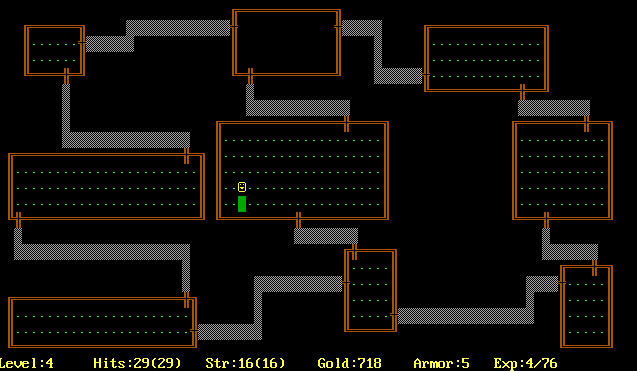
\includegraphics[scale=0.5]{Rogue.png} \\
Rogue, le jeu à l'origine des rogue-like
\end{center}

\bigbreak
\bigbreak
\bigbreak
Notre jeu sera un rogue-lite et se rapprochera donc des mécaniques habituelles de ce genre, comme par exemple des actions en temps réel et pas en tour par tour. Nous avons décidé de nous inspirer principalement de Binding of Isaac et de Enter The Gungeon. La disposition des salles sera la même que celle de Binding of Isaac, tandis que la façon de tirer et surtout le dash qui permettra d'esquiver les attaques seront inspirés de Enter The Gungeon. En soit, les mécaniques de notre jeu seront un mélange de celles de ces deux jeux. Cependant nous essaieront aussi de nous affranchir d'eux et de trouver nos propres mécaniques.

\newpage
\section{Détails et fonctionnalités du projet}

	\subsection{Détails du jeu}
	
		\subsubsection{Généralités}
\bigbreak
\bigbreak
Le projet est un jeu de type rogue-like hybride nommé \og The Believer’s Quest \fg, et sera réalisé sous Unity. Le joueur évoluera donc dans un donjon composé de 5 étages, chacun composé de plusieurs salles générées de manière aléatoire, sauf le dernier qui ne sera composé que d’une salle de boss. Pour un étage $n$, on trouvera $12 + (n - 1) * 6$ salles normales. Le joueur pourra de plus choisir le nom de son personnage.
\bigbreak
Il y aura 4 types de salles : les salles normales, les salles de coffre, le magasin, la salle du boss d’étage. Dans les salles normales, le joueur affrontera des ennemis qui, lorsqu’il les aura battus, lui fourniront de l’argent qui lui permettra d’acheter de l’équipement et des objets, et donc d’améliorer ses chances de descendre plus bas dans le donjon. Le magasin permettra au joueur d’acheter de nouvelles armes et de nouveaux objets. Les salles de coffre contiendront un coffre nécessitant une clé pour être ouvert. A l’intérieur le joueur pourra trouver une arme ou un objet aléatoire. Ce type de salle ne sera pas généré aléatoirement. Dans la salle du boss, le joueur affrontera le boss de l’étage. S’il gagne il a alors accès à l’étage suivant.

De plus, les salles normales seront générées en fonction d'un pattern choisi au hasard parmi plusieurs.
\bigbreak
La mort sera permanente, c’est-à-dire que si le joueur meurt, il perd tous ses objets et armes, sa progression est perdue et il doit tout recommencer. Cependant l’existence d’une monnaie permanente que le joueur conservera après sa mort lui permettra de débloquer de nouvelles armes dans le hub (description du hub plus bas).
\bigbreak
Les ressources graphiques et sonores seront potentiellement entièrement (ou du moins une majorité) créées par le groupe de ce projet. 
\bigbreak

		\subsubsection{But du jeu}
\bigbreak
\bigbreak
Le joueur aura pour but d’arriver au bout du donjon en battant les différents ennemis et boss qu’il rencontrera pour récupérer une coupe magique.
\bigbreak

		\subsubsection{Système monétaire}
\bigbreak
\bigbreak
Il y aura 2 types d’argent :
\begin{itemize}
\item L’or : utilisable dans le donjon et perdu après la mort. Obtenable sur tous les ennemis
\item Les diamants : utilisables dans le hub et conservés après la mort. Obtenable uniquement sur les boss
\end{itemize}
\bigbreak
\newpage
	\subsection{Structure du jeu}
		\subsubsection{Le hub}
\bigbreak
\bigbreak
Le hub est une salle où le joueur apparaît avant chaque partie. Ce dernier peut y voir les touches de mouvements par défaut. Le hub contient aussi un marchand auprès duquel le joueur peut acheter de nouvelles armes qui pourront alors apparaître dans le donjon.
\bigbreak

		\subsubsection{Les étages}
\bigbreak
\bigbreak
Il y aura 5 étages, chacun ayant leurs propres caractéristiques :
\bigbreak
\begin{itemize}
\item Étage de pierre :
\begin{itemize}
\item Ennemis : sans type secondaire
\item Charte graphique : pierre
\item Salles : 12 (2 salles de coffre + 1 magasin + 8 salles normales + 1 salle de boss)
\end{itemize}
\bigbreak
\item Étage de feu :
\begin{itemize}
\item Ennemis : type feu
\item Charte graphique : pierre en fusion
\item Salles : 18 (2 salles de coffre + 1 magasin + 14 salles normales + 1 salle de boss)
\end{itemize}
\bigbreak
\item Étage de glace :
\begin{itemize}
\item Ennemis : type glace
\item Charte graphique : glace
\item Salles : 24 (2 salles de coffre + 1 magasin + 20 salles normales + 1 salle de boss)
\end{itemize}
\bigbreak
\item Étage d’air :
\begin{itemize}
\item Ennemis : type volant
\item Charte graphique : nuages et ailes
\item Salles : 30 (2 salles de coffre + 1 magasin + 24 salles normales + 1 salle de boss)
\end{itemize}
\bigbreak
\item Étage final :
\begin{itemize}
\item Ennemis : pas d’ennemis sauf le boss
\item Charte graphique : tombeau
\item Salles : 1 salle de boss
\end{itemize}
\end{itemize}

\newpage
		\subsubsection{Les salles normales}
\bigbreak
\bigbreak
Les salles normales possèderont entre 1 et 4 portes. Les portes seront situées au milieu du mur sur lesquelles elles se situeront. Il y aura des murs et des trous dans la salle. Leur positionnement sera aléatoire mais régulé pour éviter de bloquer l’accès aux portes. Le nombre d’ennemis sera aléatoire mais la somme des poids des ennemis devra être inférieur ou égale à 7.

Des trous seront aussi générés aléatoirement à partir de l'étage 3.
\bigbreak

		\subsubsection{Les salles de coffre}
\bigbreak
\bigbreak
Ce type de salle comprendra un coffre dans lequel le joueur pourra trouver une arme ou un objet choisi « au hasard » en fonction de la rareté. Il y aura une chance que le coffre soit remplacé par un ennemi imitant un coffre (un mimic).
\bigbreak

		\subsubsection{Les magasins}
\bigbreak
\bigbreak
Dans ce type de salle, le joueur pourra acheter des armes et des objets grâce à l’or qu’il aura récupéré sur les ennemis vaincus. Le magasin vendra forcément 1 ou 2 objets de soin, 1 ou 2 clés, 2 objets et 2 armes. Le nombre de de clés et d’objets de soins sont interdépendants, c’est-à-dire que si 2 objets de soin sont en vente, alors il y aura 1 clé en vente et inversement.
\bigbreak
	\subsection{Joueur et ennemis}
		\subsubsection{Le joueur}
		\bigbreak
		\bigbreak
Le joueur contrôlera un personnage pouvant réaliser plusieurs actions :
\begin{itemize}
\item Attaquer avec son arme.
\item Utiliser l’objet équipé.
\item Se déplacer dans toutes les directions.
\item Esquiver sous la forme d’un dash (accélération rapide et courte dans la direction souhaitée). Le dash permet d’éviter les attaques et de passer au-dessus des trous.
\item Récupérer l’argent lâché par les ennemis.
\item Acheter des objets au marchand.
\end{itemize}

Le joueur possèdera 4 vies. Chaque fois qu’il sera touché par une attaque ennemie (même de la part d’un boss) il perdra 1 vie.
\bigbreak
Le joueur ne pourra posséder que 2 armes et un objet. Pour avoir une nouvelle arme ou un nouvel objet, il devra se séparer d’un article du même type en sa possession.
 \bigbreak
Une jauge d’effet sera reliée au joueur. Si elle est entièrement remplie, le joueur subit des dégâts. La jauge diminuera avec le temps jusqu’à redevenir vide.
\bigbreak

		\subsubsection{Les ennemis}
\bigbreak
\bigbreak
Il y aura plusieurs types d’ennemis. Les ennemis seront forcément d’un des 2 types principaux et pourront en plus être d’un type secondaire.
\bigbreak
Types principaux :
\begin{itemize}
\item Corps à corps : les ennemis attaquant au corps à corps.
\item A distance : les ennemis attaquant à distance.
\end{itemize}
\bigbreak
Types secondaires :
\begin{itemize}
\item Volant : les ennemis volants peuvent passer au-dessus des trous sans tomber.
\item Feu : les attaques des ennemis de feu remplissent une partie de la jauge d’effet lorsque le joueur est touché.
\item Glace : les attaques des ennemis de glace ralentiront le joueur s’il est touché.
\end{itemize}
\bigbreak 
Le type secondaire des ennemis sera déterminé par l’étage d’où ils proviennent.
\bigbreak
Lorsqu’un ennemi meurt il lâche potentiellement un ensemble de pièces dont la valeur totale est comprise entre 2 et 15 ors.
\bigbreak
On ne verra pas la vie des ennemis et ils seront de plus en plus difficiles à tuer. 
\bigbreak
Les ennemis auront un \og poids \fg \, qui permettra de réguler le nombre d’ennemis dans les salles.
\bigbreak
Les ennemis pourront réaliser les actions suivantes :
\begin{itemize}
\item Attaquer.
\item Se déplacer dans toutes les directions.
\end{itemize}
\bigbreak

		\subsubsection{Les boss}
\bigbreak
\bigbreak
Les boss seront uniques, on ne pourra pas les affronter dans les étages autres que le leur.
On pourra voir la vie des boss sous la forme d’une jauge. Lorsqu’un boss meurt il lâche forcément un ensemble de pièces dont la valeur totale est comprise entre 10 et 30 ors, et entre 1 et 4 diamants.
\bigbreak
\newpage
	\subsection{Autres}
		\subsubsection{Interface}
\bigbreak
\bigbreak
L’interface sera composée de plusieurs choses :
\begin{itemize}
\item La vie du joueur.
\item La jauge d’effet.
\item La quantité d’or possédé par le joueur (seulement dans le donjon).
\item La quantité de diamants possédés par le joueur (seulement dans le hub).
\item L’arme sélectionnée et son nombre de balles restantes (dans le chargeur et au total).
\item L’objet possédé par le joueur.
\end{itemize}
\bigbreak

		\subsubsection{Sauvegardes}
\bigbreak
\bigbreak
Le jeu sauvegardera automatiquement lorsque le joueur mourra ou lorsqu’il changera de salle.
\bigbreak

		\subsubsection{Menu pause}
\bigbreak
\bigbreak
Le menu pause donnera à l’utilisateur 5 choix :
\begin{itemize}
\item Reprendre sa partie.
\item Réinitialiser le donjon.
\item Retourner au hub.
\item Accéder aux options du jeu.
\item Quitter le jeu.
\end{itemize}

\newpage
\section{Répartition des tâches}
	\subsection{Répartition}
\bigbreak
\bigbreak
(Les croix \textcolor{red}{X} correspondent aux responsables et les X aux suppléants)
\bigbreak
\begin{tabular}{|*{5}{c|}}
	\hline
	Tâches$\backslash$ Membre & Nicolas I & Sarah & Nicolas L & Maxence \\
	\hline
	\rowcolor{Lavender}\multicolumn{5}{|c|}{ENNEMIS} \\
	\hline	
	\cellcolor{WhiteSmoke}Déplacements & & & X & \textcolor{red}{X} \\
	\hline
	\cellcolor{WhiteSmoke}Hitbox & & & \textcolor{red}{X} & X \\
	\hline
	\cellcolor{WhiteSmoke}Attaques & & \textcolor{red}{X} & & X \\
	\hline
	\rowcolor{Lavender}\multicolumn{5}{|c|}{JOUEUR} \\
	\hline
	\cellcolor{WhiteSmoke}Déplacements & & & X & \textcolor{red}{X} \\
	\hline
	\cellcolor{WhiteSmoke}Hitbox & & & \textcolor{red}{X} & X \\
	\hline
	\cellcolor{WhiteSmoke}Attaques & X & \textcolor{red}{X} & & \\
	\hline
	\rowcolor{Lavender}\multicolumn{5}{|c|}{DONJON} \\
	\hline
	\cellcolor{WhiteSmoke}Collisions mur & & X & \textcolor{red}{X} & \\
	\hline
	\cellcolor{WhiteSmoke}Génération salles & \textcolor{red}{X} & & X  & \\
	\hline
	\cellcolor{WhiteSmoke}Magasins & & X & & \textcolor{red}{X} \\
	\hline
	\rowcolor{Lavender}\multicolumn{5}{|c|}{STRUCTURE} \\
	\hline
	\cellcolor{WhiteSmoke}Graphismes & \textcolor{red}{X} & X & & \\
	\hline
	\cellcolor{WhiteSmoke}Son & & & X & \textcolor{red}{X} \\
	\hline
	\cellcolor{WhiteSmoke}Interface & & \textcolor{red}{X} & & X \\
	\hline
	\cellcolor{WhiteSmoke}Sauvegardes & \textcolor{red}{X} & & & X \\
	\hline
	\cellcolor{WhiteSmoke}Options & & \textcolor{red}{X} & X & \\
	\hline
	\rowcolor{Lavender}\multicolumn{5}{|c|}{DISTRIBUTION} \\
	\hline
	\cellcolor{WhiteSmoke}Module installation/désinstallation & X & & \textcolor{red}{X} & \\
	\hline
	\cellcolor{WhiteSmoke}Page web & X & \textcolor{red}{X} & & \\
	\hline
	\cellcolor{WhiteSmoke}Communication & X & \textcolor{red}{X} & & \\
	\hline
\end{tabular}
\bigbreak
\newpage
	\subsection{Planning}
\bigbreak
\bigbreak
\begin{tabular}{|*{4}{c|}}
	\hline
	 & Soutenance 1 & Soutenance 2 & Soutenance 3 \\
	\hline
	\rowcolor{Lavender}\multicolumn{4}{|c|}{ENNEMIS} \\
	\hline	
	\cellcolor{WhiteSmoke}Déplacements & 100\% & 100\% & 100\% \\
	\hline
	\cellcolor{WhiteSmoke}Hitbox & 0\% & 50\% & 100\% \\
	\hline
	\cellcolor{WhiteSmoke}Attaques & 30\% & 60\% & 100\% \\
	\hline
	\rowcolor{Lavender}\multicolumn{4}{|c|}{JOUEUR} \\
	\hline
	\cellcolor{WhiteSmoke}Déplacements & 100\% & 100\% & 100\% \\
	\hline
	\cellcolor{WhiteSmoke}Hitbox & 0\% & 50\% & 100\% \\
	\hline
	\cellcolor{WhiteSmoke}Attaques & 30\% & 60\% & 100\% \\
	\hline
	\rowcolor{Lavender}\multicolumn{4}{|c|}{DONJON} \\
	\hline
	\cellcolor{WhiteSmoke}Collisions mur & 50\% & 95\% & 100\% \\
	\hline
	\cellcolor{WhiteSmoke}Génération salles & 80\% & 100\% & 100\% \\
	\hline
	\cellcolor{WhiteSmoke}Magasins &  0\% & 60 \% & 100\% \\
	\hline
	\rowcolor{Lavender}\multicolumn{4}{|c|}{STRUCTURE} \\
	\hline
	\cellcolor{WhiteSmoke}Graphismes & 15\% & 50\% & 100\% \\
	\hline
	\cellcolor{WhiteSmoke}Son & 15\% & 40\% & 100\% \\
	\hline
	\cellcolor{WhiteSmoke}Interface & 20\% & 65\% & 100\% \\
	\hline
	\cellcolor{WhiteSmoke}Sauvegardes & 0\% & 50\% & 100\% \\
	\hline
	\cellcolor{WhiteSmoke}Options & 0\% & 50\% & 100\% \\
	\hline
	\rowcolor{Lavender}\multicolumn{4}{|c|}{DISTRIBUTION} \\
	\hline
	\cellcolor{WhiteSmoke}Module installation/désinstallation & 0\% & 50\% & 100\% \\
	\hline
	\cellcolor{WhiteSmoke}Page web & 80\% & 90\% & 100\% \\
	\hline
	\cellcolor{WhiteSmoke}Communication & 10\% & 50 \% & 100\% \\
	\hline
\end{tabular}
\bigbreak
\section{Aspects techniques}
	\subsection{Coût}
\bigbreak
\bigbreak
\begin{itemize}
\item Tablette de dessin Wacom Intuos Pro : environ 350 euros
\item Pointeur slider pour Diaporama : environ 15 euros
\item FL Studio : environ 200 euros
\end{itemize}

\bigbreak
	\subsection{Logiciels utilisés}
\bigbreak
\bigbreak
\begin{itemize}
\item Développement du jeu : Unity
\item Graphismes : Krita
\item Audio : FL Studio + Bosca Ceoil
\item Développement web : Atom, Notepad++
\item Cloud : Github
\end{itemize}
\bigbreak
\bigbreak
\bigbreak
	\subsection{Communication}
\bigbreak
\bigbreak
Pour la communication du projet, un site web et une page Facebook seront utilisés.
\bigbreak
Le site sera le support de la distribution du jeu. Il possédera une page de présentation du projet, une page de téléchargement, une page de news et une page de bibliographie. Les utilisateurs auront aussi la possibilité de contacter le groupe du projet. Les nouveautés et informations sur le projet seront présentées de manière complète sur le site.
\bigbreak
La page Facebook servira à une communication plus large. Des résumés, des nouveautés et informations à propos de l’avancée du projet seront transmis sur cette page.
\bigbreak

\section{Conclusion}
\bigbreak
\bigbreak
Nous sommes conscients des difficultés que nous pourrions rencontrer lors de la conception du jeu, notamment au niveau des graphismes. Néanmoins, nous sommes déterminés et motivés à réaliser notre projet jusqu'au bout et faire en sorte qu'il réponde aux attentes soulevées dans ce cahier des charges. Nous espérons de plus produire quelque chose à la fois amusant à créer et aussi très enrichissant.

\end{document}